
For now the results presented in this note are for events with no jets only. We are in process of applying ME 
method to events with one jet in the final state, the note will be updated as soon as the results become available.

The final discriminant is the likelihood ratio described in Sec.~\ref{sec:LR}.  
The LR has been evaluated for 18 different values of $m_H$ between 115 and 600 \GeVcc.
Figure~\ref{fig:lrstacks} shows the likelihood ratio distributions for $m_H$~=~130, 160, 200 and 300 \GeVcc,               
corresponding to 4.7~fb$^{-1}$. Note that the majority of backgrounds peak near $LR~=~0$ while the signal peaks near $LR~=~1$.  
It was noted in Sec.~\ref{sec:EvtSelWW} that we apply a dilepton invariant mass requirement prior to constructing the likelihood ratio. 
Figure~\ref{fig:LR_noMll} shows the likelihood ratio distribution assuming $m_{H}=160$ \GeVcc without the invariant mass requirements.
One can see from the peak at $LR~=~0$ that the Matrix Element method successfully identifies high invariant mass events as background-like, so the cut is not essential. However, by applying the cut we lose less than $1\%$ of the signal and gain significantly in processing time needed for differential cross-section calculations.

\begin{figure}[!hbtp]                                                                                         
\centering                                                                                                                                             
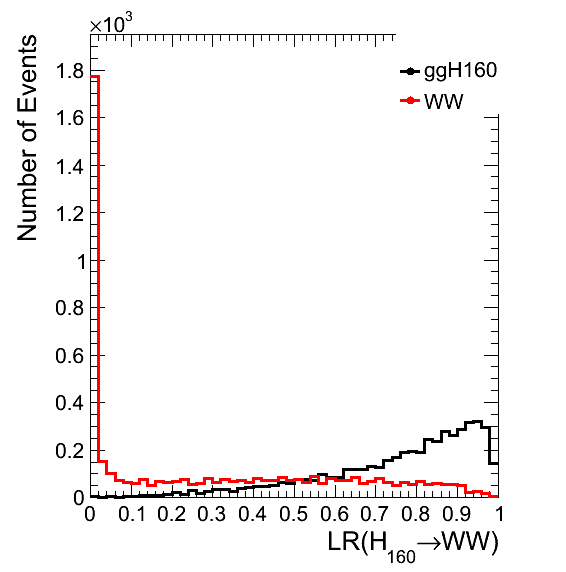
\includegraphics[width=.5\textwidth]{figures/LR_noMll.png}\\                                            
\caption{The matrix element output LR distribution after $WW$ selection but prior to $m_{ll}$ cut                      
for $m_H$=160 \GeVcc}
\label{fig:LR_noMll}                                                                                          
\end{figure}

\begin{figure}[!hbtp]                                                                                         
\centering                                                                                                    
\subfigure[]{                                                                                                 
\centering                                                                                                    
\label{subfig:lr_hm130}                                                                                       
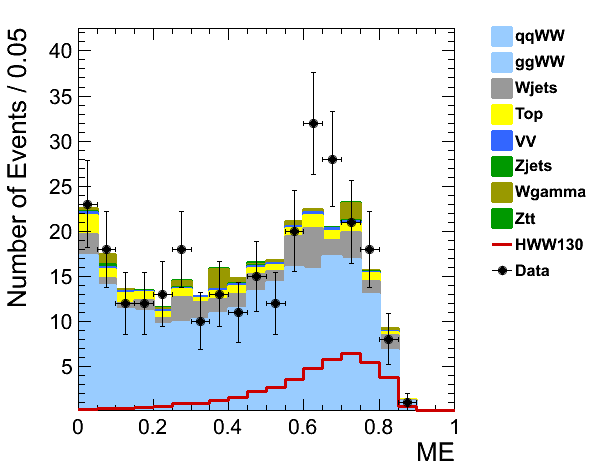
\includegraphics[width=.40\textwidth]{figures/ME_mH130_0j_of_stack_lin.png}                                                 
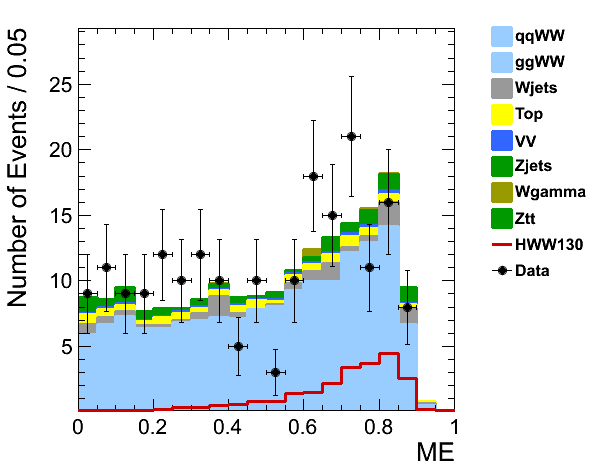
\includegraphics[width=.40\textwidth]{figures/ME_mH130_0j_sf_stack_lin.png}}                                                 
\subfigure[]{                                                                                                 
\centering                                                                                                    
\label{subfig:lr_hm160}                                                                                       
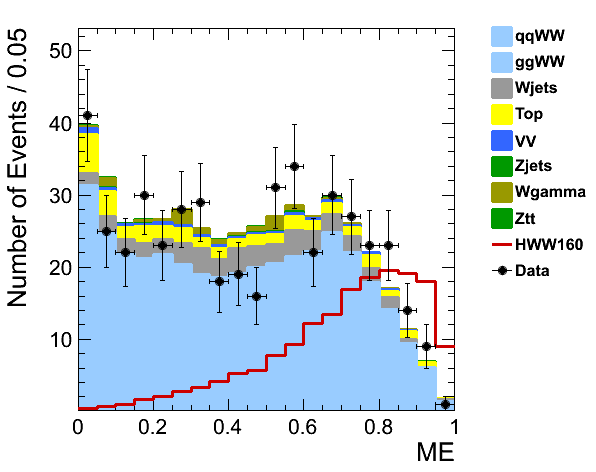
\includegraphics[width=.40\textwidth]{figures/ME_mH160_0j_of_stack_lin.png}                                                 
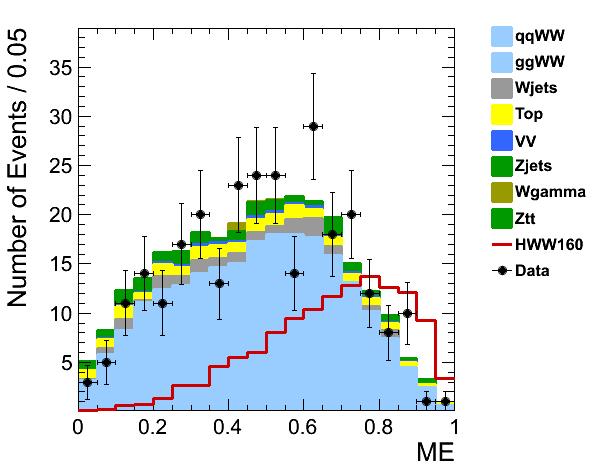
\includegraphics[width=.40\textwidth]{figures/ME_mH160_0j_sf_stack_lin.png}}                                                 
\subfigure[]{                                                                                                 
\centering                                                                                                    
\label{subfig:lr_hm200}                                                                                       
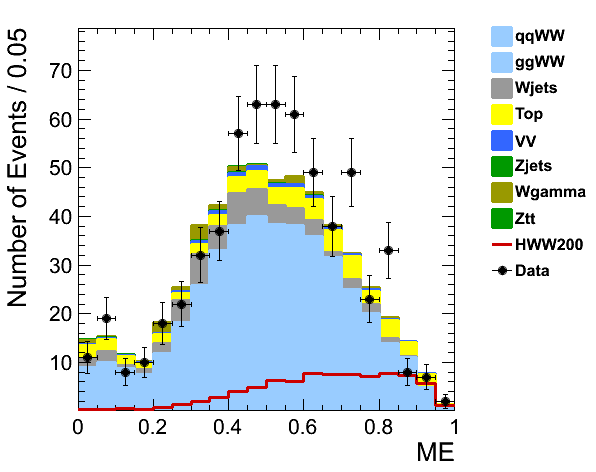
\includegraphics[width=.40\textwidth]{figures/ME_mH200_0j_of_stack_lin.png}                                                 
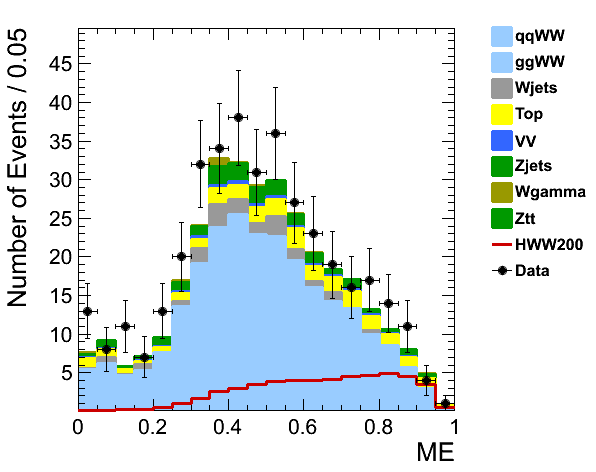
\includegraphics[width=.40\textwidth]{figures/ME_mH200_0j_sf_stack_lin.png}}                                                 
\subfigure[]{                                                                                                 
\centering                                                                                                    
\label{subfig:lr_hm300}                                                                                       
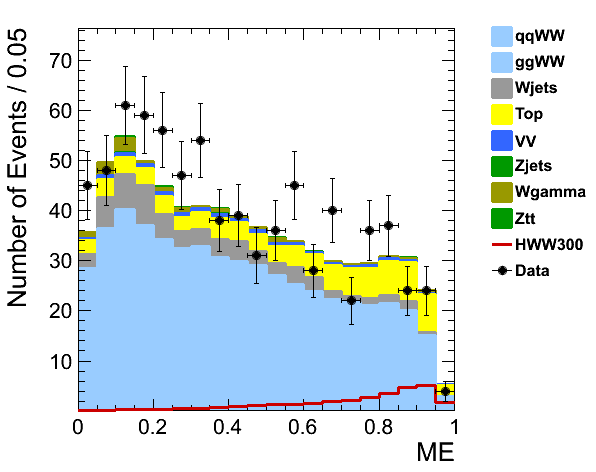
\includegraphics[width=.40\textwidth]{figures/ME_mH300_0j_of_stack_lin.png}                                                 
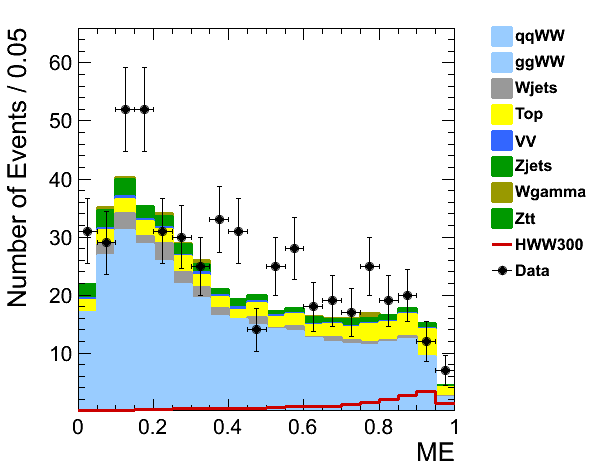
\includegraphics[width=.40\textwidth]{figures/ME_mH300_0j_sf_stack_lin.png}}\\                                                 
\caption{The matrix element based Likelihood Ratio distribution after $WW$ selection, $m_{ll}$ and $m_{T}$ cuts                      
for $m_H$=130 \GeVcc \subref{subfig:lr_hm130}, $m_H$=160 \GeVcc \subref{subfig:lr_hm160}, $m_H$=200 \GeVcc 
\subref{subfig:lr_hm200} and $m_H$=300 \GeVcc \subref{subfig:lr_hm300} in the 0-jet bin, shown separately for opposite-flavor (left)
and same-flavor (right) dilepton events.}                                            
\label{fig:lrstacks}                                                                                          
\end{figure}                      

We compute the upper limits using the shape of the LR to maximize the analysis sensitivity as described in 
Section~\ref{sec:LR}. The expected and observed upper limit at 95\%C.L. as a function of $m_H$ using the matrix element and BDT approaches are shown in 
Figure~\ref{fig:me_expected_5fb} and tabulated in \ref{tab:me_expected_5fb}. Sensitivity performance of the two methods is very similar, and provides 20-30\% improvement compared to the cut-and-count approach from \cite{ref:HWW2011smurf}. The observed 95\%C.L. exclusion range obtained using BDT and ME methods is also comparable, with slightly wider exclusion range at high $m_{H}$ for the ME method. 

To summarize, using matrix element based approach in $H\rightarrow WW \rightarrow l^{+}l^{-}\nu\bar{\nu}$ 0-jet bin analysis we exclude Standard Model Higgs boson in the 128--275 GeV mass range, with expected exclusion range of 128--235 GeV at 95\% C.L. For comparison, BDT expected and observed exclusion ranges in the 0-jet channel are similar: 128--230 GeV and 128--240 GeV, respectively.  

\begin{figure}[!hbtp]
\centering
\subfigure[]{
\centering
\label{subfig:me_exp_5fb}
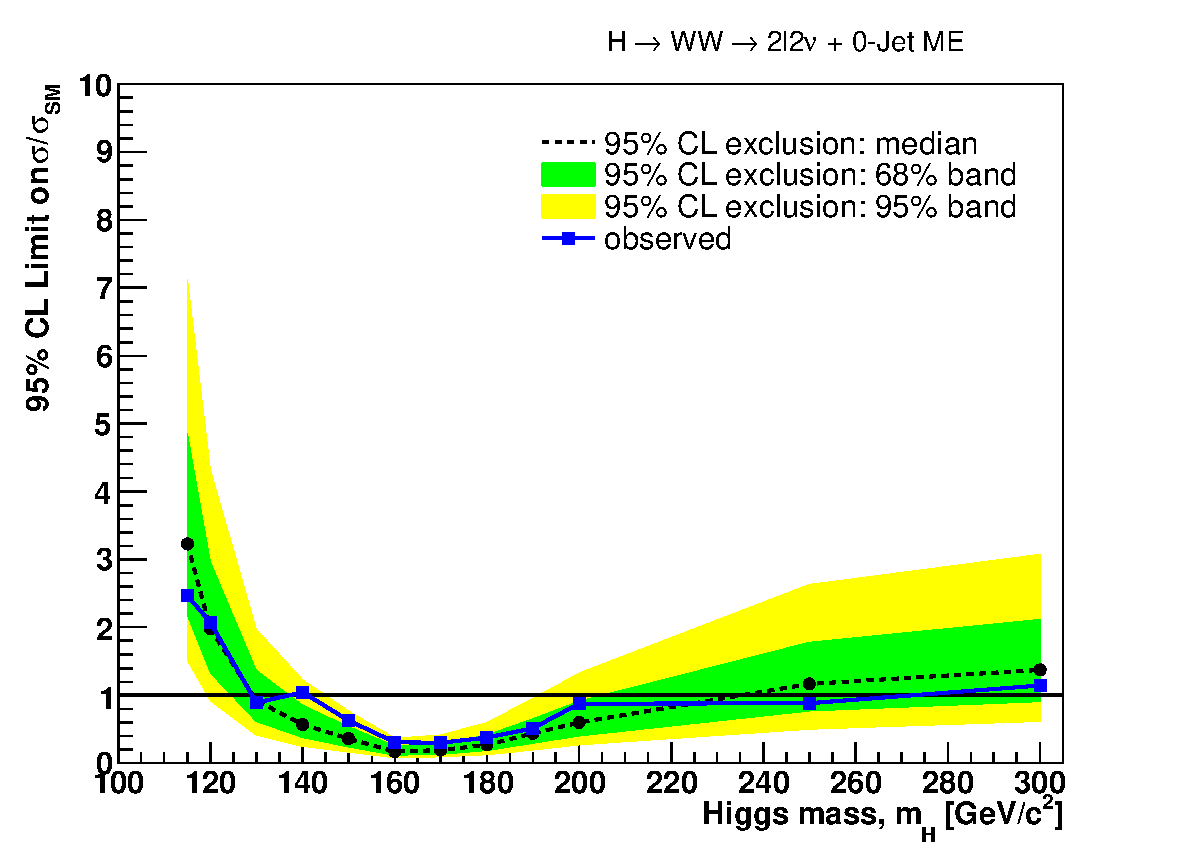
\includegraphics[width=.8\textwidth]{figures/limit_0j_shape_me_shapesyst.pdf}}
\subfigure[]{
\centering
\label{subfig:bdt_exp_5fb}
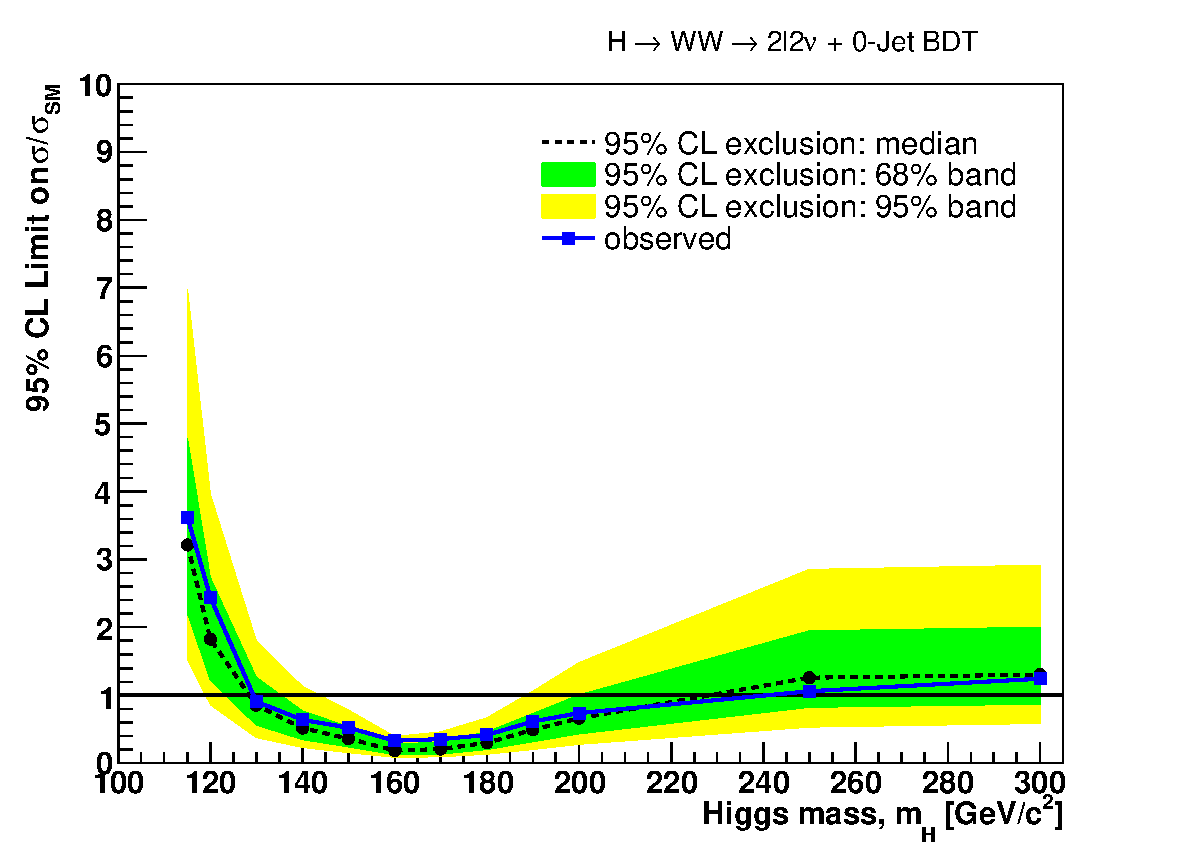
\includegraphics[width=.8\textwidth]{figures/limit_0j_shape_bdt_shapesyst.pdf}}
\caption{ 
Multivariate shape analysis expected and observed upper limits at 95\% C.L. for 4.7~fb$^{-1}$ data using the 
matrix elemement \subref{subfig:me_exp_5fb} and BDT \subref{subfig:bdt_exp_5fb}. Limits are for 0-jet bin only. } 
\label{fig:me_expected_5fb}
\end{figure}

\begin{table}
\begin{center}
\begin{tabular}{c c c c c c}
\hline\hline
 Higgs Mass   & Observed & Median expected & Expected range for 68\% & Expected range for 95\%   \\
\hline
\multicolumn{5}{c} {Matrix Element Method} \\
\hline
115 & 2.5 & 3.2 & [2.2, 4.8] & [1.5, 7.1] \\
120 & 2.1 & 2.0 & [1.3, 3.0] & [0.9, 4.3] \\
130 & 0.9 & 0.9 & [0.6, 1.4] & [0.4, 2.0] \\
140 & 1.0 & 0.6 & [0.4, 0.9] & [0.2, 1.2] \\
150 & 0.6 & 0.4 & [0.2, 0.5] & [0.2, 0.8] \\
160 & 0.3 & 0.2 & [0.1, 0.3] & [0.1, 0.4] \\
170 & 0.3 & 0.2 & [0.1, 0.3] & [0.1, 0.4] \\
180 & 0.4 & 0.3 & [0.2, 0.4] & [0.1, 0.6] \\
190 & 0.5 & 0.4 & [0.3, 0.7] & [0.2, 0.9] \\
200 & 0.9 & 0.6 & [0.4, 0.9] & [0.3, 1.3] \\
250 & 0.9 & 1.2 & [0.8, 1.8] & [0.5, 2.6] \\
300 & 1.1 & 1.4 & [0.9, 2.1] & [0.6, 3.1] \\
350 & 1.2 & 1.2 & [0.8, 1.9] & [0.6, 2.8] \\
400 & 1.1 & 1.4 & [0.9, 2.1] & [0.6, 3.2] \\
450 & 1.3 & 2.1 & [1.4, 3.2] & [0.9, 4.8] \\
500 & 2.3 & 3.2 & [2.2, 4.9] & [1.5, 7.4] \\
550 & 3.0 & 4.9 & [3.3, 7.7] & [2.2, 11.7] \\
600 & 5.0 & 7.8 & [5.0, 12.1] & [3.3, 19.2] \\
\hline
\multicolumn{5}{c} {BDT Based} \\
\hline
115 & 3.6 & 3.2 & [2.2, 4.8] & [1.5, 7.0] \\
120 & 2.4 & 1.8 & [1.2, 2.7] & [0.9, 4.0] \\
130 & 0.9 & 0.9 & [0.6, 1.3] & [0.4, 1.8] \\
140 & 0.6 & 0.5 & [0.3, 0.8] & [0.2, 1.1] \\
150 & 0.5 & 0.4 & [0.2, 0.5] & [0.2, 0.8] \\
160 & 0.3 & 0.2 & [0.1, 0.3] & [0.1, 0.4] \\
170 & 0.4 & 0.2 & [0.1, 0.3] & [0.1, 0.5] \\
180 & 0.4 & 0.3 & [0.2, 0.5] & [0.1, 0.7] \\
190 & 0.6 & 0.5 & [0.3, 0.7] & [0.2, 1.1] \\
200 & 0.7 & 0.7 & [0.4, 1.0] & [0.3, 1.5] \\
250 & 1.1 & 1.3 & [0.8, 2.0] & [0.5, 2.9] \\
300 & 1.2 & 1.3 & [0.9, 2.0] & [0.6, 2.9] \\
350 & 1.1 & 1.2 & [0.8, 1.8] & [0.5, 2.7] \\
400 & 1.3 & 1.3 & [0.9, 2.1] & [0.6, 3.0] \\
450 & 1.4 & 1.9 & [1.3, 2.9] & [0.8, 4.3] \\
500 & 1.7 & 2.8 & [1.9, 4.3] & [1.3, 6.5] \\
550 & 2.9 & 4.3 & [2.9, 6.6] & [1.9, 10.3] \\
600 & 3.8 & 6.5 & [4.2, 10.2] & [2.8, 15.6] \\
\hline\hline
\end{tabular}
\end{center}
\caption{Multivariate shape analysis Bayesian expected and observed upper limits at 95\% C.L.
for 4.7~fb$^{-1}$ of data using the BDT and matrix element outputs for the 0-jet bin.}
% corresponding to Figure~\ref{fig:me_expected_1fb}.}
\label{tab:me_expected_5fb}
\end{table}

